\chapter{Data Sample, Event Selection, and Jet Definitions}\label{ch:data_and_event_selection}

\section{Data Sample}\label{sec:data}
This analysis uses the entirety of the 2015 and 2016 ATLAS datasets, comprising \linebreak $36.1~fb^{-1}~(\pm2.1\%)$ of integrated luminosity, with $\sqrt{s}=13~TeV$.
A \textit{good runs list} (GRL) is used to select only those blocks of luminosity which pass basic detector quality criteria~\cite{data-grl}.

\section{Trigger}\label{sec:trigger}
Events are required to pass an $H_{T}$-based trigger, where $H_{T}$ is the scalar sum of the $p_{T}$ of all jets in an event.
The jets used for the calculation of $H_{T}$ in the trigger are level-one jets with $p_{T}>100~GeV$.
To pass the trigger, an event must have $H_{T}>1~TeV$.
Figure~\ref{fig:trigger_efficiency} shows the trigger efficiency versus large-$R$ jet $p_{T}$ threshold for events with $\geq4$ and $\geq5$ large-$R$ jets.
For events with five or more large-$R$ jets, the trigger efficiency is $100\%$ when the jet $p_{T}$ threshold is $200~GeV$ or above.
For events with four or more jets, an additional requirement on the leading jet $p_{T}$ is needed to ensure full trigger efficiency at this jet-$p_{T}$ threshold.
For the $\geq4$-jet regions, the leading jet will be required to have a $p_{T}$ of at least $400~GeV$.

\begin{figure}[!ht]
    \centering
    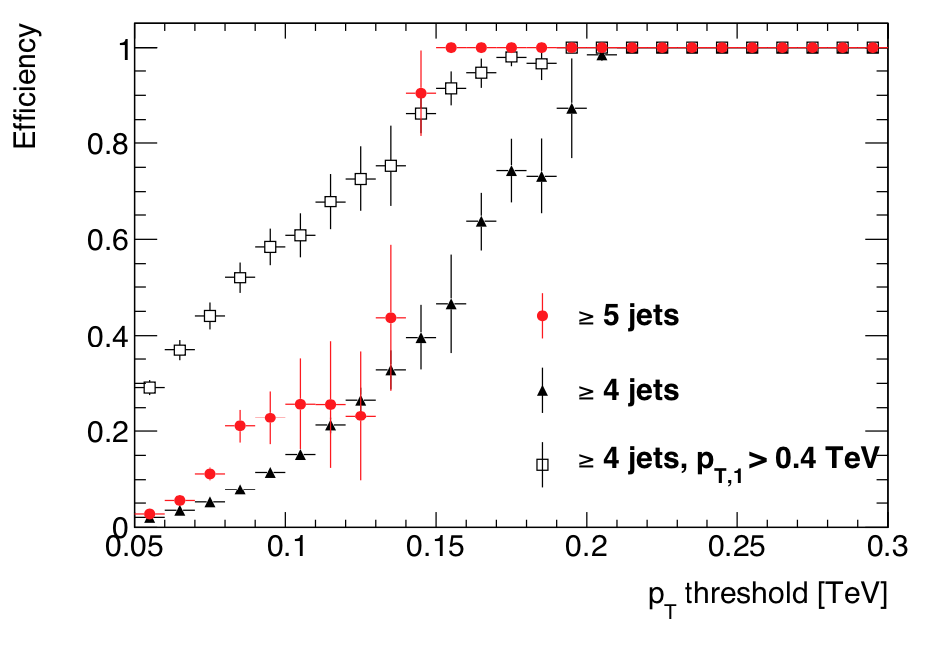
\includegraphics[width=0.9\textwidth]{data_trigger_efficiency}
    \caption{Trigger efficiency versus large-$R$ jet $p_{T}$ threshold for events with $\geq4$ and $\geq5$ large-$R$ jets.
    For events with $\geq4$ large-$R$ jets, and additional requirement of leading-jet $p_{T}>400~GeV$ ensures $100\%$ trigger efficiency.
    }
    \label{fig:trigger_efficiency}
\end{figure}

\section{Event selection}\label{sec:event_selection}

Events considered by this analysis must meet the following pre-selection criteria:

\begin{itemize}
    \item In the list of good luminosity blocks in the GRL as described in~\ref{sec:data}.
    \item No errors in the LAr or tile calorimeters or the inner detector when the events were measured
    \item Pass the $H_{T}$ trigger as described in~ref{sec:trigger}.
    \item At least one primary vertex from at least two tracks with $p_{T}>400~MeV$ each
    \item At least one large-$R$ jet (see~\ref{sec:jet_definitions}) with $p_{T}>440~GeV$
\end{itemize}

\section{Jet definitions, b-tagging, and b-matching}\label{sec:jet_definitions}

In this analysis, two different types of jets are defined.
Large-$R$ jets are reconstructed using the anti-$k_{T}$ algorithm with $R=1.0$, and trimming is applied.
Large-$R$ jets are required to have $p_{T}>200~GeV$.
The following parameters are used in large-$R$ jet reconstruction:

\begin{itemize}
    \item $R=1.0$
    \item $R_{sub-jet}=0.2$
    \item $f_{p_{T}}=0.05$
\end{itemize}

Small-$R$ jets are reconstructed using the anti-$k_{T}$ algorithm with $R=0.4$.
To be considered for b-tagging, a small-R jet must have $p_{T}$ of at least $50~GeV$ and $|\eta|$ less than $2.5$.
The fixed-efficiency $70\%$ working point is used for $b$-tagging.

For details of how jets are reconstructed, trimmed, and calibrated, as well as the definition of different jet parameters, see chapter~\ref{ch:jets}.
The algorithm used to tag b-jets is described in chapter~\ref{subsec:jet_b_tagging} as well as~\cite{b-jet-perf-1,b-jet-perf-2}.

Large-$R$ jets found to be within $\Delta R=1.0$ of a $b$-tagged small-$R$ jet in the same event are referred to as $b$-matched jets.
Those large-$R$ jets not within $\Delta R=1.0$ of a $b$-tagged small-$R$ jet are called non-$b$-matched.
The distinction in terminology between $b$-tagged and $b$-\textit{matched} is important enough to restate for clarity.
When referring to the presence or absence of a $b$-tagged jet \textit{within an event}, the terms $b$-tag, $b$-veto, and $b$-inclusive are used.
When referring to the proximity of an \textit{individual large-$R$ jet} to a $b$-tagged small-$R$ jet, the terms $b$-matched and non-$b$-matched are used.

The control, validation, and signal regions defined in section~\ref{sec:region_defs} can be segmented into $b$-tag and $b$-veto regions.
Events with at least one $b$-tagged small-$R$ jet are considered $b$-tag events, while those without are labelled as $b$-veto.
When $b$-tagging is not part of the selection requirements for a region, it is called a $b$-inclusive region.

